\documentclass[a4paper,10pt]{article}
\usepackage[T1]{fontenc}
\usepackage[utf8]{inputenc}
\usepackage[english]{babel}
\usepackage{lmodern}
\usepackage[top=1.6cm,bottom=1.8cm,left=1.9cm,right=1.9cm]{geometry}
\usepackage{titlesec,enumitem,xcolor,graphicx,lastpage,fancyhdr}
\usepackage{fontawesome5}
\usepackage[hidelinks]{hyperref}

\hypersetup{colorlinks=true,urlcolor=blue!70!black,linkcolor=blue!70!black}
\pagestyle{fancy}\fancyhf{}\renewcommand{\headrulewidth}{0pt}
\fancyfoot[C]{\small\color{gray}Page \thepage\ of \pageref{LastPage}}
\setlength{\parindent}{0pt}

\titleformat{\section}{\large\bfseries\color{blue!70!black}}{}{0em}{}[\vspace{-0.7em}\rule{\textwidth}{0.5pt}]
\titlespacing{\section}{0pt}{9pt}{5pt}
\setlist[itemize]{leftmargin=1.1em,itemsep=2pt,topsep=2pt,parsep=0pt}
\newcommand{\role}[4]{\vspace{3pt}\noindent\hspace{0.6em}\parbox[t]{0.38\textwidth}{\raggedright\textbf{#1}}\hfill\parbox[t]{0.58\textwidth}{\raggedleft\textit{#2}}\\{\textit{#3}\hfill\textit{#4}}\vspace{1pt}}

\begin{document}
\noindent
\begin{minipage}[t]{0.78\textwidth}
\vspace{0pt}
{\huge\bfseries Prabhavit Gupta}\\[8pt]
{\small \faPhone\ +39-351-610-7807 \quad \faEnvelope\ \href{mailto:prabhavitg@gmail.com}{prabhavitg@gmail.com} \quad \faLinkedin\ \href{https://www.linkedin.com/in/prabhavit/}{Linkedin} \quad \faMapMarker*\ Venice, Italy}
\end{minipage}\hfill
\begin{minipage}[t]{0.18\textwidth}
\vspace{0pt}\raggedleft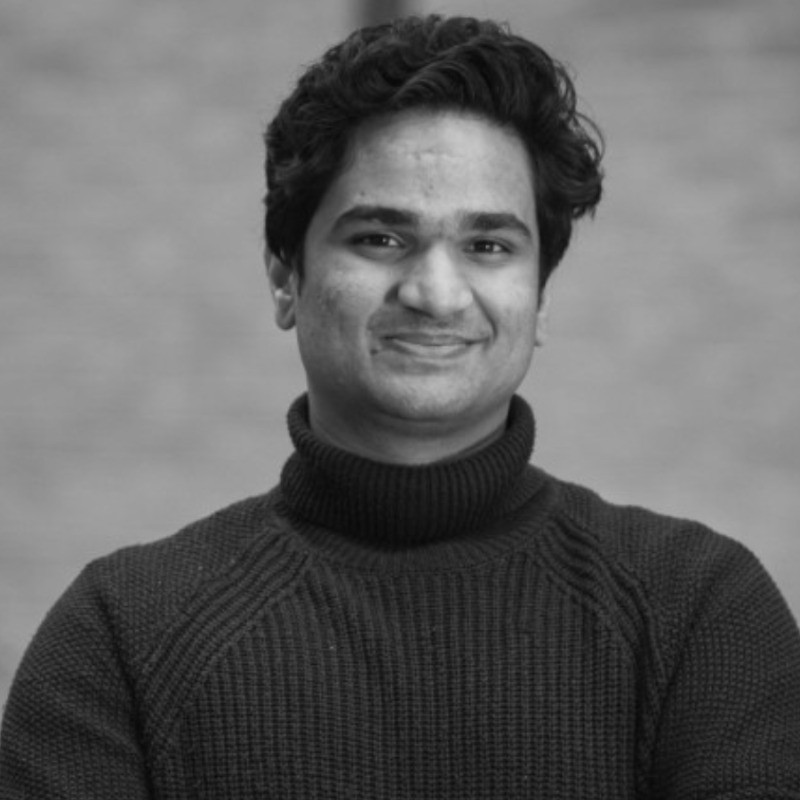
\includegraphics[width=2.3cm,height=2.3cm,keepaspectratio]{photo.jpg}
\end{minipage}

\section{Career Summary}
\begin{itemize}
\item Robotics \& Automation Software Engineer with a mechanical engineering foundation and hands-on experience in software validation, testing automation, and industrial systems.
\item Proficient in Python, C++, and Bash scripting for test harness development, motion validation, and hardware-software integration across automated manufacturing systems.
\item Proven background combining Politecnico di Milano engineering training with production automation, troubleshooting, and rigorous quality assurance protocols.
\end{itemize}

\section{Technical Skills}
\begin{itemize}
\item \textbf{Robotics \& Automation} -- Robotics Software Validation, Toolpath Testing, Additive Manufacturing Systems, Industrial Automation, Motion Validation
\item \textbf{Programming \& Scripting} -- Python, C++, JavaScript, Bash, SQL, Git, Linux
\item \textbf{Testing \& QA} -- Software Test Automation, Hardware-in-the-Loop Validation, Regression Testing, Bug Tracking, Postman
\item \textbf{Protocols \& Architecture} -- REST APIs, Modbus/Serial, Microservices, Docker, Technical Documentation
\end{itemize}

\section{Visa \& Language}
\begin{itemize}
\item \textbf{Language} -- Italian (Conversational / Intermediate), English (Fluent / Professional), Hindi (Native)
\item \textbf{Work Authorization} -- European Long Term Residence Permit - No Sponsorship required. Driving License (Patente B).
\end{itemize}

\section{Professional Experience}
\role{\href{https://flowspace.co}{FlowSpace.co}}{Automation Lead Developer (Full time, Freelance)}{London, UK}{Mar 2024 -- Ongoing}
\begin{itemize}
\item \textbf{Technical \& Systems Responsibilities:}
\begin{itemize}[label=--]
\item Developed automated test suites and validation harnesses in Python and Playwright, reducing software regression bugs by 40\%.
\item Engineered real-time telemetry and error logging pipelines to capture edge-case system faults and improve runtime reliability.
\item Created comprehensive technical test plans, interface contract documentation, and validation protocols for engineering teams.
\end{itemize}
\item \textbf{Quality Assurance \& Operations:}
\begin{itemize}[label=--]
\item Supervised platform migration and continuous integration workflows ensuring 99.9\% uptime across production services.
\item Performed root cause analysis on software exceptions and collaborated with R\&D to deploy permanent system patches.
\end{itemize}
\item \textit{Tools: Python, Linux, Bash, Playwright, REST APIs, Docker, Git, Jira}
\end{itemize}

\role{Urlink}{Systems Automation Engineer}{Milan, Italy}{Jul 2023 -- Feb 2024}
\begin{itemize}
\item Developed Python validation scripts to verify data integrity across connected operational hardware and cloud databases.
\item Collaborated with field engineering teams to resolve tier-2 software issues, delivering diagnostic tooling and custom patches.
\item Documented system behaviors, automated regression checks, and conducted validation tests before production rollouts.
\end{itemize}

\role{UltraStrategy}{Automation Developer}{Remote, Germany}{Sep 2022 -- Jun 2023}
\begin{itemize}
\item Automated manufacturing and operational data extraction pipelines using modular Python scripts and REST endpoints.
\item Implemented automated validation scripts enforcing strict schema adherence and anomaly detection.
\end{itemize}

\section{Education}
\role{Politecnico di Milano}{M.Sc. in Management Engineering (Digital Business \& ICT)}{Milan, Italy}{2020 -- 2023}
\role{Thapar Institute of Engineering and Technology}{B.E. in Mechanical Engineering}{Punjab, India}{2014 -- 2018}

\end{document}
